\chapter{Kjarneðlisfræði}

\section{Stærð kjarnans}

\begin{tcolorbox}
\begin{definition}
Lítum á frumefni $X$ með massatölu $A$ og sætistölu $Z$ þar sem að mismunurinn á fjölda róteinda og nifteinda er $k$ (hleðslan). Við táknum þá frumefnið með rithættinum:
\begin{align*}
    \ce{^{A}_{Z}X^{k}}
\end{align*}
\end{definition}
\end{tcolorbox}

\begin{figure}[H]
    \centering
    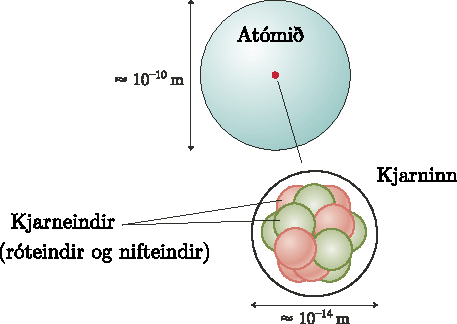
\includegraphics[scale = 1]{figures/atomid-staerd.pdf}
\end{figure}

\begin{tcolorbox}
\begin{theorem}
Lítum á kjarna frumefnis sem hefur massatölu $A$ og sætistölu $Z \geq 2$. Þá er geisli kjarnans gefin með:
\begin{align*}
    r = r_0 A^{1/3}, \hspace{0.5cm} \text{þar sem} \hspace{0.5cm} r_0 = \SI{1.2}{fm}.
\end{align*}
\end{theorem}
\end{tcolorbox}

\textbf{Útleiðsla:} Eðlismassi kjarnans er fastur (róteindirnar og nifteindirnar pakka sér svo þétt saman að eðlismassinn helst óbreyttur). Kjarninn er þar með eins og ein stór kúla með sama eðlismassa og ein kjarneind. Ef við gerum þá nálgun að $m_n \approx m_p \approx u$ þá höfum við að:
\begin{align*}
    \rho_{\text{kjarni}} = \frac{m_n}{\frac{4\pi}{3}r_0^3}
\end{align*}
Þar sem að $r_0$ er geisli nifteindar. Þar sem að eðlismassi kjarnans helst óbreyttur þá ályktum við að:
\begin{align*}
    \frac{Am_n}{\frac{4\pi}{3}r^3} = \rho_{\text{kjarni}} = \frac{m_n}{\frac{4\pi}{3}r_0^3} \implies r = Ar_0^3 \implies r = r_0 A^{1/3}.
\end{align*}
\qed

\section{Geislavirkni}

\begin{figure}[H]
    \centering
    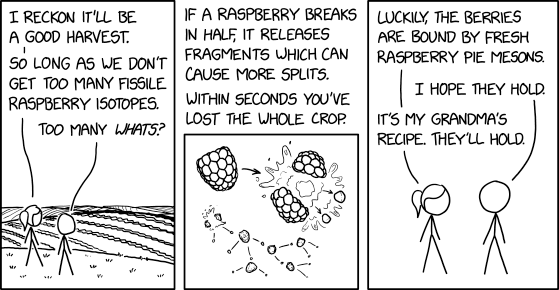
\includegraphics[width = 0.5\textwidth]{figures/fissile_raspberry_isotopes.png}
\end{figure}

\begin{figure}[H]
    \centering
    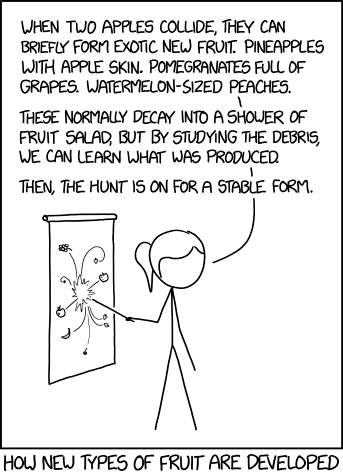
\includegraphics[width = 0.2\textwidth]{figures/fruit_collider.png}
\end{figure}

\begin{tcolorbox}
\begin{definition}
Látum $N(t)$ tákna heildarfjölda frumeinda í sýni af geislavirku efni. Heildarfjöldi frumeinda hrörnar þá (yfir í önnur frumefni) samkvæmt hrörnunarhreyfingunni: 
\begin{align*}
    \frac{dN}{dt} = -\lambda N,
\end{align*}
þar sem $\lambda$ er stuðull sem kallast hrönunarstuðull og táknar líkur þess að geislavirka efnið hrörni.
\end{definition}
\end{tcolorbox}

\begin{tcolorbox}
\begin{theorem}
Lítum á sýni af geislavirku efni sem hefur hrörnunarstuðul $\lambda$. Í upphafi inniheldur sýnið $N_0$ frumeindir af geislavirka efninu. Þá er heildarfjöldi frumeinda eftir tímann, $t$, gefinn með:
\begin{align*}
    N(t) = N_0 e^{-\lambda t}.
\end{align*}
\end{theorem}
\end{tcolorbox}

\textbf{Útleiðsla:} Geislavirka efnið uppfyllir hrörnunarhreyfinguna:
\begin{align*}
    \frac{dN}{dt} = -\lambda N \implies \frac{dN}{dt} + \lambda N = 0.
\end{align*}
Margföldum síðan báðar hliðar með $e^{\lambda t}$ og pillum síðan afleiðuna af til að fá:
\begin{align*}
    \frac{dN}{dt}e^{\lambda t} + \lambda e^{\lambda t}N = 0 \implies \frac{d}{dt}\left( Ne^{\lambda t}  \right) = 0 \implies Ne^{\lambda t} = C \implies N(t) = Ce^{-\lambda t}
\end{align*}
Þar sem $C$ er fasti sem að ákvarðast af upphafsskilirðinu $N(0) = N_0 = C$ svo við höfum sýnt að:
\begin{align*}
    N(t) = N_0 e^{-\lambda t}.
\end{align*} 

\qed

\begin{tcolorbox}
\begin{theorem}
Helmingunartími geislavirka efnisins er þá gefinn með:
\begin{align*}
    \tau = \frac{\ln(2)}{\lambda}.
\end{align*}
\end{theorem}
\end{tcolorbox}

\textbf{Útleiðsla:} Við höfum þá að:
\begin{align*}
    N(\tau) = \frac{N_0}{2} \implies N_0e^{-\lambda \tau} =  \frac{N_0}{2} \implies e^{-\lambda \tau} = \frac{1}{2} \implies -\lambda \tau = \ln(\frac{1}{2}) \implies \tau = \frac{\ln(2)}{\lambda}.
\end{align*}
\qed


\begin{figure}[H]
    \centering
    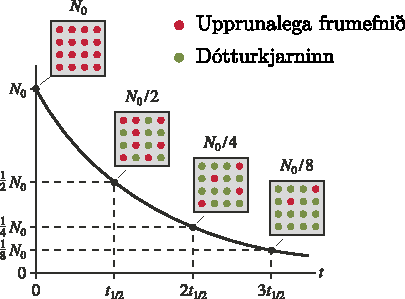
\includegraphics[scale = 1]{figures/hrornun.pdf}
    \caption{Heildarfjöldi frumeinda af geislavirku efni hrörnar með tíma yfir í stöðugan dótturkjarna.}
\end{figure}

\begin{tcolorbox}
\begin{definition}
Við skilgreinum \textbf{geislavirkni}, $G(t)$, frá geislavirku efni með heildarfjölda frumeinda, $N(t)$, sem stærðina:
\begin{align*}
    G(t) = -\frac{dN}{dt}.
\end{align*}
\end{definition}
\end{tcolorbox}

\begin{tcolorbox}
\begin{theorem}
Lítum á sýni af geislavirku efni sem hefur hrörnunarstuðul $\lambda$. Í upphafi inniheldur sýnið $N_0$ frumeindir af geislavirka efninu. Þá er geislavirkni frumefnisins gefin með:
\begin{align*}
    G(t) = G_0e^{-\lambda t}, \hspace{1cm} G_0 = N_0 \lambda.
\end{align*}
\end{theorem}
\end{tcolorbox}

\textbf{Útleiðsla:} Við athugum að:
\begin{align*}
    G(t) = -\frac{dN}{dt} = -\frac{d}{dt}\left( N_0e^{-\lambda t} \right) = N_0 \lambda e^{-\lambda t} = G_0 e^{-\lambda t}.
\end{align*}
\qed

Það ber að nefna á þessum tímapunkti að stærðin sem að við mælum oftast (og er auðveldast að mæla) er $G_0$ (það er að segja geislavirknina frá geislavirku sýni einmitt þegar að mælingin er framkvæmd). Þessi stærð er það mikið notuð að hún hefur fengið sína eigin SI-einingu sem er kennd við franska eðlisfræðingin Henri Becquerel (sem hlaut Nóbelsverðlaunin í eðlisfræði árið 1903 ásamt hjónunum Marie og Pierre Curie). Hún er skilgreind þannig að:

\begin{align*}
    \left[ G_0 \right] = \SI{}{\frac{\text{fjöldi frumeinda sem hrörnar}}{s}} = \SI{}{Bq}
\end{align*}

En þið hafið eflaust heyrt um kjarnorkusprengjurnar Little Boy og Fat Man sem var varpað yfir japönsku stórborgnir Hiroshima og Nagasaki árið 1945. Þið hafið eflaust líka heyrt af ýmsum kjarnorkuslysum sem hafa orðið í gegnum árin eins og í Chernobyl í Úkraínu árið 1986 og í Fukushima í Japan árið 2011. Þið vitið þá eflaust líka að það getur verið gríðarlega skaðlegt fyrir manneskjur að verða fyrir of mikilli geislavirkni. Helstu læknisfræðilegu annmarkar sem að því fylgja eru aukin tíðni krabbameina. Við viljum því hafa einhvern læknisfræðilegan grundvöll\footnote{Í læknisfræðilegum skilningi getur eftirfarandi vefsíða verið fróðleg: \href{https://gr.is/liffraedileg-ahrif-jonandi-geislunar/}{https://gr.is/liffraedileg-ahrif-jonandi-geislunar/}} til þess að tala um skaðsemi geislavirkra efna. Ef þið hafið einhverntímann handleikið geislunarmæli (Geiger-mælir) þá vitið þið að hann mælir svokölluð sívert (\si{Sv}) en það er kennt við sænska heilbrigðiseðlisfræðinginn Rolf Maximilian Sievert. Reyndar mæla flestir geislunarmælar \si{\mu Sv/klst}. Ástæðan fyrir þessu er sú að það skiptir okkur læknisfræðilega ekkert voðalega miklu máli hversu mikil geislavirknin er heldur hversu orkurík hún er (það er sú orka sem fer í að eyðileggja erfðaefnið okkar). 


\begin{tcolorbox}
\begin{definition}
Lítum á hlut sem hefur massa $m$ og verður fyrir geislun með heildarorku $\Delta E$. Við skilgreinum þá \textbf{geislunarálag} geislunarinnar sem stærðina:
\begin{align*}
    H = \frac{w\Delta E}{m}
\end{align*}
Þar sem $w$ er svokallaður \textbf{geislunarstuðull} og ákvarðast af læknisfræðilegri skaðsemi geislunarinnar:
\begin{align*}
    w_\alpha = 20, \hspace{1cm} w_\beta = 1, \hspace{1cm} w_\gamma = 1
\end{align*}

Geislunarálag er mælt í mælieiningunni sívert $\left[ H \right] = \frac{\si{J}}{\si{kg}} = \si{Sv}$.
\end{definition}
\end{tcolorbox}

Það getur síðan verið fróðlegt að rýna í eftirfarandi töflu (sjá líka xkcd: \href{https://xkcd.com/radiation/}{https://xkcd.com/radiation/}) til þess að átta sig betur á geislunarálaginu sem að fylgir mismunandi athöfnum:

\begin{table}[H]
    \centering
    \begin{tabular}{|c|l|}
    \hline
        \SI{50}{n Sv} & Að sofa í sama rúmi og önnur manneskja \\ \hline
       \SI{100}{nSv}  & Borða banana (kalín) \\ \hline
       \SI{250}{n Sv}  & Að fara í gegnum öryggishlið á flugvelli \\ \hline
       \SI{1}{\mu Sv}  & Liggja í sólbaði í einn dag \\ \hline
       \SI{6}{\mu Sv}  & Dagsferð til Pripyat með viðkomu hjá Chernobyl kjarnaofninum \\ \hline
       \SI{10}{\mu Sv}  & Röntgenmyndir af tönnum í tannlæknaheimsókn \\ \hline
       \SI{20}{\mu Sv}  & Flugferð frá Íslandi til Danmerkur.  \\ \hline
       \SI{1}{m Sv}  & Árleg bakgrunnsgeislun á \href{https://gr.is/wp-content/uploads/2016/09/natturulegt_geislaalag_norraent.pdf}{Íslandi}  \\ \hline
       \SI{2}{m Sv}  & Heilasneiðmynd (CT scan)  \\ \hline
       \SI{6}{m Sv}  & Árlegt geislunarálag flugáhafnarmeðlima  \\ \hline
       \SI{50}{m Sv}  & Hámarksgeislun á ári fyrir geislunarstarfsfólk \\ \hline
       \SI{1}{Sv}  & Geislaveiki (getur verið banvænt)  \\ \hline
       \SI{8}{Sv}  & Banaskammtur   \\ \hline
    \end{tabular}
    \caption{Skammtastærðir af geislunarálagi}
    \label{table:geislun}
\end{table}

\section{Kjarnaorka og stöðugleiki frumefna}

\begin{tcolorbox}
\begin{definition}
Við skilgreinum frumeindamassann, $u$, þannig að kolefnissamsætan $\ce{^{12}C}$ hafi massann $12\text{u}$ en það þýðir að:
\begin{align*}
    \SI{1}{u} = \SI{1.6605e-27}{kg}.
\end{align*}
\end{definition}
\end{tcolorbox}

\begin{table}[H]
    \centering
    \begin{tabular}{|l|c|c|c|c|}
    \hline
        Eind & Tákn & Massi $(\text{u})$ & Massi $(\si{\frac{MeV}{c^2}})$ & Massi $(\si{kg})$ \\ \hline \hline
        Rafeind & $e$ & $0,00055$ & \SI{0.511}{} & \SI{9.109e-31}{kg}  \\ \hline
        Róteind & $p$ & $1,00728$ & \SI{938.3}{} & \SI{1.673e-27}{kg} \\ \hline
        Nifteind & $n$ & $1,00866$ & \SI{939.6}{} & \SI{1.675e-27}{kg} \\ \hline
        Alpha-ögn & $\alpha$ & $4,002602$ & \SI{3728}{} & \SI{6.64e-27}{kg} \\ \hline
    \end{tabular}
    \caption{Massi helstu öreindanna. Frumeindamassinn er $\SI{1}{u} = \SI{1.6605e-27}{kg} = \SI{931.49}{\frac{MeV}{c^2}}$.}
\end{table}

Hér erum við að sjálfsögðu þá að tala um kyrrstöðumassa eindanna en þá samkvæmt Einstein vitum við að það er alveg eins hægt að tala um tilheyrandi kyrrstöðuorku (margföldum bara með $c^2$ til að fá $E_0 = m_0 c^2$). Þar sem að það er erfitt að vinna með stærðir af stærðargráðunni \SI{e-27}{} þá vilja öreindafræðingar miklu frekar vinna með eininguna $\si{MeV/c^2}$ í þeim einingum þá verða massarnir:
\begin{align*}
    E_u = \text{u}c^2 = \SI{931.49}{MeV}.
\end{align*}
Þannig að stundum skrifum við:
\begin{align*}
    1 \text{u} = \SI{1.6605e-27}{kg} = \SI{931.49}{MeV/c^2}.
\end{align*}

\begin{tcolorbox}
\begin{definition}
Lítum á efnahvarf af gerðinni:
\begin{align*}
    \ce{X} \to \ce{Y} + \ce{Z}
\end{align*}
Þá er \textbf{kjarnaorkan}, $\Delta E$, sem að losnar í þessu hvarfi er gefin með:
\begin{align*}
    \Delta E = \Delta m c^2 = \left(m_X - m_Y - m_Z\right)c^2
\end{align*}
\end{definition}
\end{tcolorbox}

\section{Mismunandi gerðir af jónandi geislun (\boldmath $\alpha$, \boldmath $\beta$ og \boldmath $\gamma$ geislun)}

Í þessari undirgrein ætlum við að kynna til sögunnar alla þá geislun sem að getur losnað í kjarnahvörfum.

\subsection{\boldmath $\alpha$-geislun}

Ef að frumeindakjarninn er of stór til þess að sterki kjarnakrafturinn geti haldið kjarnanum saman þá mun kjarninn ekki vera stöðugur. Það verða því einhverjar líkur (skammtafræði) á því að $\alpha$-ögn losni til þess að mynda stöðugri dótturkjarna. Í stuttu máli er $\alpha$-geislunin afleiðing af því hvað gerist þegar að sterki kjarnakrafturinn er ekki nógu sterkur.

\begin{tcolorbox}
\begin{definition}
$\alpha$-geislun einkennist af eftirfarandi hrörnunarhvarfi:
\begin{align*}
    \ce{^{A}_{Z}X ->[\alpha] ^{A-4}_{Z-2}Y + ^{4}_{2}\alpha}^{+2}
\end{align*}
Í rauninni er $\alpha$-ögnin bara rafeindalaus helíumkjarni $\ce{^4_2He^{+2}}$.
\end{definition}
\end{tcolorbox}

Kjarnaorkan sem að losnar við $\alpha$-geislun fer nánast öll í hreyfiorku $\alpha$-agnarinnar (sérstaklega ef upprunalega frumefnið, $X$, er með mjög háa sætistölu, $Z$). Við höfum þá að:
\begin{align*}
    K_{\alpha} \approx \Delta E  = \left( m_X - m_Y - m_\alpha \right)c^2
\end{align*}
Mismunandi efni hafa síðan mismunandi líkur á því hversu líklegt er að frumefnið $X$ geisli frá sér $\alpha$-ögn. Eina leiðin til þess að útskýra almennilega hvað það er nákvæmlega sem að ákvarðar helmingunartíma frumefnanna er með því að nota skammtafræði og þá sér í lagi að skoða líkur þess að $\alpha$-agnirnar smjúgi í gegn um Coulomb-þröskuldinn.



\subsection{\boldmath $\beta$-geislun}

Í stuttu máli þá verður $\beta$-geislun þegar að veiki kjarnakrafturinn er ekki nógu sterkur til þess að halda kjarnanum saman. Í löngu máli er þetta hinsvegar algjör hausverkur til þess að setja sig inn í. 

\begin{tcolorbox}
\begin{definition}
Það eru til tvær gerðir af $\beta$-geislun:
\begin{enumerate}[label = \textbf{(\roman*)}]
    \item $\boldsymbol{\beta^-}$ geislun: \hspace{0.4cm} $\ce{^{A}_{Z}X ->[\beta^-] ^{A}_{Z+1}Y + e^{-} + \overline{\nu}_e}$
    \item $\boldsymbol{\beta^+}$ geislun: \hspace{0.4cm} $\ce{^{A}_{Z}X ->[\beta^+] ^{A}_{Z-1}Y + e^{+} + \nu_e}$
\end{enumerate}
\end{definition}
\end{tcolorbox}

Það kemur í ljós að $\beta^-$ geislun er mun algengari heldur en $\beta^+$ geislun. Í $\beta^-$ geislun þá breytist ein nifteind í eina róteind og eina rafeind (og andeind tilheyrandi fiseindar rafeindarinnar). Hinsvegar í $\beta^+$ geislun þá breytist ein róteind í eina nifteind og eina jáeind (og eina tilheyrandi fiseind rafeindarinnar). Það væri því alveg eins hægt að setja þetta fram með eftirfarandi hætti:

\begin{tcolorbox}
$\beta$-geislun einkennist af eftirfarandi tveimur kjarnahvörfum:
\begin{align*}
\ce{n ->[\beta^-] p^+ + e^- + \overline{\nu}_e}, \hspace{1cm} \ce{p^+ ->[\beta^+] n + e^+ + \nu_e}
\end{align*}
\end{tcolorbox}

Kjarnaorkan sem að losnar í $\beta$-geislun fer nánast öll í hreyfiorku $\beta$-eindarinnar (sem er rafeindin sem að losnar) er því gefin með:
\begin{align*}
    K_\beta \approx \Delta E = \left( m_X - m_Y \right)c^2
\end{align*}

Tæknilega séð er til ein geislun í viðbót vegna veika kjarnakraftsins sem að kallast rafeindarhremming (táknað með $\text{EC}$ sem er skammstöfun fyrir Electron Capture) og einkennis af eftirfarandi kjarnahvarfi:
\begin{tcolorbox}
\begin{align*}
\ce{^{A}_{Z}X+ + e^- ->[\text{EC}] ^{A}_{Z-1}Y + \nu_e } \hspace{0.5cm} \text{þ.e.} \hspace{0.5cm} \ce{p^+ + e^- ->[\text{EC}] n + \nu_e }
\end{align*}
\end{tcolorbox}






\subsection{Gamma-geislun}

Er einfaldasta geislunin til þess að útskýra. Þetta gerist þegar að frumefni í örvuðu ástandi geisla frá sér ljóseindum og fara niður á lægra orkustig:

\begin{tcolorbox}
\begin{definition}
$\gamma$-geislun einkennis af eftirfarandi hrönunarhvarfi:
\begin{align*}
    \ce{^{A}_{Z}X ->[\gamma] ^{A}_{Z}X + \gamma}
\end{align*}
Í rauninni er $\gamma$-eindin bara ljóseind.
\end{definition}
\end{tcolorbox}
Kjarnaorkan sem að losnar fer þá (nánast öll) í ljóseindina sem að fær þá orku
\begin{align*}
    \Delta E_{\text{atóm}} = E_{\text{ljóseind}} = hf
\end{align*}
þar sem $f$ er tíðni ljóseindarinnar sem myndaðist og $h = \SI{6.626e-34}{J.s}$ er fasti Plancks.

\newpage

\section{Dæmi}

\subsection*{Dæmatími 35: Kjarna- og öreindafræði: Kjarninn}

\begin{tcolorbox}
Frumeindarmassi frumefna er táknaður með $A$. Sætistala frumefna er táknuð með $Z$. Heildarfjöldi róteinda í kjarnanum er þá $Z$ og heildarfjöldi nifteinda er $A-Z$. Mismunurinn á fjölda róteinda og nifteinda er táknaður með $k$ (ef $k$ er jákvæð eru fleiri róteindir heldur en rafeindir, en ef $k$ er neikvæð eru fleiri rafeindir heldur en róteindir). Fyrir frumefnið $X$ er þetta gefið til kynna með því að skrifa:
\begin{align*}
    \ce{^{A}_{Z}X^{k}}
\end{align*}
Hægt er að ákvarða geisla kjarnans, $r$, út frá frumeindarmassanum samkvæmt:
\begin{align*}
    r = r_0A^{1/3}, \hspace{1cm} \text{þar sem} \hspace{0.5cm} r_0 = \SI{1.2}{fm}.
\end{align*}
Ef $A$ er frumeindamassinn þá er massi frumeindarinnar $m = Au$ þar sem $u = \SI{1.66e-27}{kg}$.
\end{tcolorbox}

\begin{enumerate}[label = \textbf{(\alph*)}]

\item[\textbf{(37.19)}] Hversu margar rafeindir, róteindir og nifteindir eru í eftirfarandi frumefnum: \\
\begin{enumerate*}[label = \textbf{(\alph*)}]
    \item \ce{^{10}_{5}B^{0}}
    \item \ce{^{13}_{7}N^{+}}
    \item \ce{^{17}_{8}O^{+++}}
    \item \ce{^{132}_{54}Xe^{0}}
\end{enumerate*}

\item[\textbf{(37.21)}] Skrifið niður frumefnin á myndunum hér fyrir neðan á forminu: \ce{^{A}_{Z}X^{k}}.

\begin{figure}[H]
    \centering
    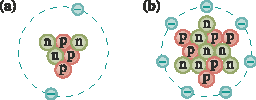
\includegraphics[scale = 1.5]{figures/atomic-struc.pdf}
\end{figure}

\item[\textbf{(37.23)}] Ákvarðið massa, geisla og eðlismassa kjarnans í eftirfarandi frumefnum: \begin{enumerate*}[label = \textbf{(\alph*)}]
    \item $\ce{^{7}_{3}Li}$
    \item $\ce{^{207}_{82}Pb}$
\end{enumerate*}

\item[\textbf{(37.25)}] Skoðum gullsamsætuna $\ce{^{197}_{79}Au}$. \begin{enumerate*}[label = \textbf{(\alph*)}]
    \item Hversu margar rafeindir, róteindir og nifteindir eru í samsætunni?
    \item Hver er geisli kjarnans?
    \item Hver er eðlismassi kjarnans?
    \item Eðlismassi gulls er \SI{11400}{kg/m^3}. Hversu mörgum sinnum eðlismeiri er kjarninn?
\end{enumerate*}

\begin{comment}
\item[\textbf{(37.25)}] \begin{enumerate}[label = \textbf{(\alph*)}]
    \item Úransamsætan, $\ce{^{235}_{92}U}$, er mikið notuð í kjarnorkuverum. Hver er eðlismassi úrankjarnans?
    \item Stjörnur er kyntar með kjarnasamruna sem að breytir vetni í helín. Þegar stjörnurnar hafa klárað vetnisbirgðir sínar þá er helst tvennt í stöðunni: Ef stjarnan er tiltölulega massalítil $(\leq 8 M_{\text{sól}})$ þá lærir stjarnan að kynda kjarnasamrunan með helíni og tútnar síðan út og verður þá rauður dvergur (þetta verða örlög sólarinnar okkar eftir 5 milljarða ára) sem að breytist síðan að lokum í hvítan dverg þegar að hún kólnar. Hinsvegar, ef að hún er of massamikil þá er ekkert annað í stöðunni fyrir hana en að taka frekjukast og springa sem sprengistjarna. Kjarni stjörnunnar fellur þá saman undan gríðarlegum þyngdarkröftum og stjarnan endar ævi sína sem nifteindastjarna. Hver yrði geisli nifteindastjörnu sem hefði jafn mikinn massa og sólin okkar?
    
    
    \item Í dag er geisli sólarinnar \SI{6.96e8}{m} og hún snýst einn hring um sjálfa sig á \SI{27}{daga} fresti. Hversu oft myndi hún snúast um sjálfa sig á einum degi ef að hún myndi breytast í nifteindastjörnu?
\end{enumerate}
\end{comment}

\begin{comment}
\item[\textbf{(47.39)}] Stjörnur er kyntar með kjarnasamruna sem að breytir vetni í helín. Þegar stjörnurnar hafa klárað vetnisbirgðir sínar þá er helst tvennt í stöðunni: Ef stjarnan er tiltölulega massalítil $(\leq 8 M_{\text{sól}})$ þá lærir stjarnan að kynda kjarnasamrunan með helíni og tútnar síðan út og verður þá rauður dvergur (þetta verða örlög sólarinnar okkar eftir 5 milljarða ára) sem að breytist síðan að lokum í hvítan dverg þegar að hún kólnar. Hinsvegar ef að hún er of massamikil þá er ekkert annað í stöðunni fyrir hana en að taka frekjukast og springa sem sprengistjarna. Kjarni stjörnunnar fellur þar næst saman undan gríðarlegum þyngdarkröftum og flestar sprengistjörnur enda síðan ævina sína sem nifteindastjörnur. En það nafn er fengið því að 
\begin{enumerate*}[label = \textbf{(\alph*)}]
    \item Ímyndum okkur að sólin okkar myndi skyndilega falla saman í nifteindastjörnu (hún mun ekki gera það). Hver yrði þá geisli hennar? Gerið ráð fyrir að hún tapi ekki neinum massa við þetta ferli.
    \item Í dag snýst sólin um sjálfa sig einu sinni á \SI{27}{daga} fresti. Hver yrði hornhraði nifteindastjörnunnar?
\end{enumerate*}
\end{comment}

\end{enumerate}

\begin{tcolorbox}
\begin{enumerate*}[label = ]
  \item \textbf{(37.21)} $\ce{^{6}_{3}Li^{+}}$, $\ce{^{13}_{6}C^{-}}$
  \item \textbf{(37.23)} $m_{{\ce{Li}}} = \SI{1.2e-26}{kg}$, $r_{{\ce{Li}}} = \SI{2.3}{fm}$, $\rho_{{\ce{Li}}} = \SI{2.3e17}{\frac{kg}{m^3}}$, $m_{{\ce{Pb}}} = \SI{3.4e-25}{kg}$, $r_{{\ce{Pb}}} = \SI{7.1}{fm}$, $\rho_{{\ce{Pb}}} = \SI{2.3e17}{\frac{kg}{m^3}}$,
  \item \textbf{(37.25)} $(n,p,e) = (118,79,79)$, $r_{\ce{Au}} = \SI{7.0}{fm}$, $\rho_{\ce{Au}} = \SI{2.7e17}{\frac{kg}{m^3}}$, $\SI{2.4e13}{}$ sinnum eðlisþéttari.
\end{enumerate*}
\end{tcolorbox}

\newpage

\subsection*{Dæmatími 36: Kjarna- og öreindafræði: Tvístrun}

\begin{tcolorbox}
Stöðuorka rafkraftsins er $U_k = \frac{kq_1 q_2}{r}$. Ef krafturinn er aðdráttarkraftur þá er formerkið á stöðuorkunni neikvætt en ef krafturinn er fráhrindikraftur er formerkið á stöðuorkunni jákvætt. Í flestum tvístrunardæmum er hægt að hunsa áhrif afstæðiskenningarinnar. Reyndar á Rutherford sjálfur að hafa sagt um afstæðiskenninguna: \textit{``Oh, that stuff. We never bother with that in our work.''}
\end{tcolorbox}

\begin{enumerate}[label = \textbf{(\alph*)}]

\item[\textbf{(37.43)}] Skrautleg leið til þess að segja $\ce{^{4}_{2}He^{+2}}$ er að kalla það $\alpha$-ögn (sagnfræðileg ástæða). Nú er $\alpha$-ögn með orku \SI{6.24}{MeV} skotið beint í áttina að kjarna óþekkts frumefnis, $\ce{^{A}_{Z}X}$. $\alpha$-ögnin kemst næst í \SI{6.00}{fm} fjarlægð frá kjarna frumefnisins áður en að hún tvístrast og snýr við. Hvert er frumefnið?

\item[\textbf{(37.44)}] Yfir hvaða spennumun þarf að hraða $\alpha$-eind ($\ce{^{4}_{2}He^{+2}}$) úr kyrrstöðu þannig að hún rétt nær að snerta yfirborð kolefniskjarnans $\ce{^{12}_{6}C}$ sem hefur þvermál \SI{5.50}{fm}?

\item[\textbf{(37.45)}] Hver þarf hraði róteindar að vera til þess að hún rétt nái að snerta yfirborð súrefniskjarnans $\ce{^{16}_{8}O}$?

\begin{comment}
\item[\textbf{(37.46)}] Til þess að hefja kjarnaklofnun í kjarnorkuveri er róteind skotið inn í kjarna úrsansamsætunnar $\ce{^{235}_{92}U}$. Til þess að róteindin geti klofið kjarnan þarf hún að hafa hreyfiorku \SI{1783}{MeV} þegar að hún stingur sér leið inn í kjarnann (hið minnsta). \begin{enumerate}[label = \textbf{(\alph*)}]
    \item Hver þarf hraði róteindarinnar að vera hið minnsta?
    \item Yfir hvaða spennumun þarf að hraða róteindinni úr kyrrstöðu til þess að hún fái þennan hraða?
\end{enumerate}
\end{comment}

\item[\textbf{(37.46)}] Í öreindahröðlum er róteindum skotið beint inn í kjarna massamikilla frumefna í von um að hefja kjarnahvörf. Í einni tiltekinni tilraun í stóra sterkeindahraðlinum (LHC) í CERN er róteindum skotið inn í blýkjarna (\ce{^{207}_{82}Pb}). Til þess að kljúfa blýkjarnann þá þarf róteindin að hafa (að minnsta kosti) hreyfiorku \SI{20}{MeV} þegar að hún kemur að yfirborði blýkjarnans. Hver þarf hraði róteindanna að vera í upphafi til þess að ná fram þessum kjarnahvörfum?

\end{enumerate}

\begin{tcolorbox}
\begin{enumerate*}[label = ]
  \item \textbf{(37.43)} $\ce{^{27}_{13}Al}$.
  \item \textbf{(37.44)} $\SI{1.6}{MV}$.
  \item \textbf{(37.45)} $\SI{0.09}{}c$.
  \item \textbf{(37.46)} $\SI{0.27}{}c$.
\end{enumerate*}
\end{tcolorbox}

\newpage

\subsection*{Dæmatími 37: Kjarna- og öreindafræði: Bindiorka og kjarnorka}

\begin{tcolorbox}
\begin{minipage}{\linewidth}
\begin{wrapfigure}{r}{2in}
\vspace{-0.5cm}
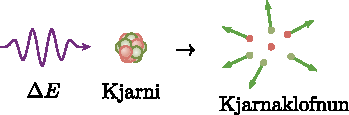
\includegraphics[width = 2in]{figures/kjarnaklofnun.pdf}
\end{wrapfigure}

Kjarnanum er haldið saman af sterka kjarnakraftinum. Ef að við viljum kljúfa kjarnann og þar með leysa úr læðingi kjarnaorkuna þá þurfum við að bæta við orku:
\begin{align*}
    \Delta E = \Delta m c^2
\end{align*}
Kjarnasamruni er síðan ferlið þegar að við setjum kjarneindirnar aftur í kjarnann (þá losnar orka). \\
\end{minipage}
Það eru síðan helst þrjár gerðir af geislavirkni sem að gefa frá sér orkuríka geislun:
\begin{multicols}{2}
\begin{itemize}
    \item $\alpha$-geislun: $\ce{^{A}_{Z}X ->[\alpha] ^{A-4}_{Z-2}Y + ^{4}_{2}\alpha}^{+2}$
    \item $\gamma$-geislun: $\ce{^{A}_{Z}X ->[\gamma] ^{A}_{Z}X + \gamma}$
    \item $\beta^{-}$-geislun: $\ce{^{A}_{Z}X ->[\beta^-] ^{A}_{Z+1}Y + e^{-} + \overline{\nu}_e}$
    \item $\beta^{+}$-geislun: $\ce{^{A}_{Z}X ->[\beta^+] ^{A}_{Z-1}Y + e^{+} + \nu_e}$
\end{itemize}
\end{multicols}
Ath. Í þessum dæmakafla gætuð þið þurft að nota efnafræðilegu upplýsingarnar í viðhenginu.
\end{tcolorbox}

\begin{enumerate}[label = \textbf{(\alph*)}]

\item[\textbf{(42.25)}] Ákvarðið óþekktu samsæturnar, $\ce{^{A}_{Z}X}$, í eftirfarandi efnahvörum: \\

\begin{enumerate*}[label = \textbf{(\alph*)}]
    \item $\ce{X -> ^{224}_{88}Ra + ^{4}_{2}\alpha}$
    \item $\ce{X -> ^{207}_{82}Pb + e^{-} + \overline{\nu}_e}$
    \item $\ce{X -> ^{40}_{19}K + e^{+} + \nu_e}$
    \item $\ce{X -> ^{60}_{28}Ni + \gamma}$
\end{enumerate*}

\phantom{.}

\begin{enumerate*}[label = \textbf{(\alph*)}]
    \setcounter{enumii}{4}
    \item $\ce{^{230}_{90}Th -> X + ^{4}_{2}\alpha}$
    \item $\ce{^{35}_{16}S -> X + e^{-} + \overline{\nu}_e}$
    \item $\ce{^{24}_{11}Na -> ^{24}_{12}Mg + e^{-} + \overline{\nu}_e -> X+\gamma}$.
\end{enumerate*}

\item[\textbf{(42.29)}] Hver er heildarorkan (í $\si{MeV}$) sem að losnar við það að eftirfarandi samsætur hrörna: \begin{enumerate*}[label = \textbf{(\alph*)}]
    \item $^{233}_{92}U$ \item $^{14}_{12}C$.
\end{enumerate*}

\item[\textbf{(42.64)}] Það tók menn mjög langan tíma að átta sig á tilvist nifteindarinnar (James Chadwick ,,uppgötvaði`` nifteindina árið 1932 meira en 20 árum eftir að Rutherford uppgötvaði róteindina og kjarnann). Ástæðan fyrir þessu var sú að $\beta^-$ hrörnun blekkti menn. Í $\beta^-$ hrörnun eru það rafeindir sem að losna úr kjarnanum svo að ályktunin sem að menn drógu frá því var að þá hlyti rafeindin að hafa verið þar inni í kjarnanum allann tímann! Við getum litið á sem svo að $\beta^-$ hrörnun samanstandi af efnahvarfinu: $n \to p^+ + e^-$ (massi andnifteindarinnar er svo lítill að við getum hunsað hann). \begin{enumerate*}[label = \textbf{(\alph*)}]
    \item Hver er heildarorkan sem að losnar í $\beta^-$-hrörnun?
    \item Með því að skoða ,,áreksturinn`` með skriðþunga- og orkuvarðveislu samkvæmt takmörkuðu afstæðiskenningunni er hægt að sýna að \SI{99.9}{\percent} af orkunni sem að losnar í efnahvarfinu fer í hreyfiorku rafeindarinnar. Hver verður þá hraði rafeindarinnar sem losnar?
\end{enumerate*}

\item[\textbf{(42.51)}] Englendingurinn Engilbert elskar að fá sér engiferte með engri mjólk. Engilbert er meðvitaður um loftlagsbreytingar og er alltaf að reyna að minnka kolefnissporið sitt. Honum hefur dottið það snilldarráð í hug að hita teið sitt með geislavirku samsætunni radíum, $\ce{^{223}_{88}Ra}$ sem að hrörnar samkvæmt efnahvarfinu $\ce{^{223}_{88}Ra ->[\alpha] ^{219}_{86}Rn + ^{4}_{2}\alpha^{2+}}$. Hann tekur því \SI{100}{mL} af vatni við \SI{18}{\degree C} (eðlisvarmi vatns er \SI{4190}{\frac{J}{kg.K}}). Engilbert hendir síðan radíummola ofan í vatnið í vel einangruðu íláti. Hver þarf massi radíummolans að vera til þess að orkan sem að losnar við hrönunina nái að hita vatnið upp að suðu?

\end{enumerate}

\begin{tcolorbox}
\begin{enumerate*}[label = ]
  \item \textbf{(42.29)} $\SI{4.91}{MeV}$, $\SI{0.156}{MeV}$
  \item \textbf{(42.64)} $\SI{0.773}{MeV}$, $v_e = 0,917c$, $v_p = 0,00128c$.
  \item \textbf{(42.51)} $\SI{15.8}{\mu g}$.
\end{enumerate*}
\end{tcolorbox}

\newpage

\subsection*{Dæmatími 38: Kjarna- og öreindafræði: Geislavirkni}

\begin{tcolorbox}
Geislavirk efni eru óstöðug og hrörna yfir í stöðugri efni. Það er háð geislavirka efninu hversu líkleg sú hrörnun er. Breytingin í heildarfjölda einda, $N$, fylgir þá hrörnunarhreyfingu:
\begin{align*}
    \frac{dN}{dt} = -\lambda N \implies N(t) = N_0e^{-\lambda t}
\end{align*}
Þar sem $\lambda$ er stuðull sem kallast hrönunarstuðull og táknar líkur þess að geislavirka efnið hrörni. Við segjum þá að geislavirknin frá þessu sýni sé gefin með:
\begin{align*}
    G(t) = -\frac{dN}{dt} = \lambda N_0 e^{-\lambda t} = G_0 e^{-\lambda t}.
\end{align*}
Geislavirkni hefur eininguna $\left[ G \right] = \si{Bq}$ (Henri Becquerel til heiðurs). Líffræðilegt geislunarálag hlutar með massa $m$ sem verður fyrir geislun með orku $\Delta E$ er skilgreint sem:
\begin{align*}
    H = \frac{w\Delta E}{m}
\end{align*}
Þar sem að $w$ er svokallaður geislunarstuðull og er háður geisluninni ($w_\alpha = \SI{20}{}$, $w_\gamma = 1$ og $w_\beta = 1$). Geislunarálag er mælt í einingunni $\left[ H \right] = \si{Sv}$ (sænska heilbrigðiseðlisfræðingnum Rolf Maximilian Sievert til heiðurs).

\end{tcolorbox}

\begin{enumerate}[label = \textbf{(\alph*)}]


\item[\textbf{(42.18)}] Geislavirka samsætan baríum, $\ce{^{131}_{56}Ba}$, hefur helmingunartíma upp á \SI{12}{daga}. Marie Curie skoðar hrörnun á \SI{250}{\mu g} sýni yfir nokkra daga. Hver er massi sýnisins eftir
\begin{enumerate*}[label = \textbf{(\alph*)}]
    \item \SI{1}{dag}
    \item \SI{10}{daga}
    \item \SI{100}{daga}
\end{enumerate*}

\item[\textbf{(42.23)}] Helmingunartími geislavirku samsætunnar $\ce{^{60}_{27}Co}$ er \SI{5.27}{ár}. Irène Joliot-Curie mælir \SI{3.50e9}{Bq} geislavirkni frá tilteknu kóbaltsýni. Hver er massi sýnisins?

\item[\textbf{(42.49)}] Lítill slúbbert í ónefndum bekk sullar niður lausn af geislavirka efninu sesín, $\ce{^{137}_{55}Cs}$, í efnafræðitíma hjá Má. Þetta þýðir því miður að það þarf að loka skólanum og bíða eftir því að geislavirknin frá sýninu lækki niður í gildi sem að geislavarnir ríkisins telja sómasamlegt fyrir stofnun af þessari stærð. Starfsmaður frá geislavörnum ríkisins mælir \SI{2.0e10}{Bq} geislavirkni í efnafræðistofunni skömmu eftir slysið. Hann veit að sesín hrörnar með $\beta^-$ hrörnun og að helmingunartími þess er \SI{30}{ár}. Hann ályktar því að geislavirknin megi mest vera \SI{9.25e8}{Bq}. Hversu lengi þarf að loka Menntaskólanum?

\item[\textbf{(42.58)}] Plútóníum samsætan $\ce{^{239}_{94}Pu}$ hefur helmingunartíma $\tau_{\!_{\ce{Pu}}} = \SI{2.412e4}{ár}$ og hrörnar með $\alpha$-geislun. Hreyfiorka $\alpha$-agnanna sem að losna í kjarnahvarfinu er \SI{5.2}{MeV}. Í þessu dæmi ætlum við að skoða líffræðilegu hættuna sem að því fylgir að anda að sér litlu rykkorni af plútóníumi með þvermál \SI{1}{\mu m}. Eðlismassi plútóníums er $\rho_{\!_{\ce{Pu}}} = \SI{19800}{kg/m^3}$.
\vspace{-0.2cm}
\begin{enumerate}[label = \textbf{(\alph*)}]
    \item Hversu margar Plútóníum frumeindir eru í einu rykkorni?
    \item Hver er geislavirkni (\si{Bq}) rykkornsins í upphafi?
    \item Hér er geislavirknin ekki mikil og hreyfiorka $\alpha$-agnana er heldur ekki mikil þar að auki sem að drægni þeirra er ekki nema \SI{50}{\mu m}. Hinsvegar þá munu allar $\alpha$-agnirnar sem að losna ná að skemma lungnavefi líkamans því plútóníum rykkornið er fast í lungunum. Lungnavefirnir hafa um það bil sama eðlismassa og vatn, þ.e.~$\rho_{\text{lungu}} = \SI{1000}{kg/m^3}$. Hversu mikið er geislunarálgið á einu ári?
\end{enumerate}

\end{enumerate}

\begin{tcolorbox}
\begin{enumerate*}[label = ]
  \item \textbf{(42.18)} $\SI{236}{\mu g}$, $\SI{140}{\mu g}$, $\SI{0.78}{\mu g}$.
  \item \textbf{(42.23)} $\SI{83.6}{\mu g}$.
  \item \textbf{(42.49)} $\SI{133.5}{ár}$.
  \item \textbf{(42.58)} $\SI{2.61e10}{atóm}$, $\SI{23.7}{mBq}$, $\SI{191}{\frac{MSv}{ári}} \gg \SI{1}{\frac{mSv}{ári}}$
\end{enumerate*}
\end{tcolorbox}

\newpage